\newpage
\section{Umsetzung}

Das Ziel ist das Erkennen und Labeln von Objekten in einer AR Umgebung, durch Image Based Objekt Detection.

\subsection{Design des Vorgang der Objekt Ernennung}

Im Folgenden werden die Arbeitsschritte einer Detection beschrieben.

Wenn der Nutzer das Signal gibt, beginnt die Detection. Als Erstes wird ein Foto mit der Kamera der AR Brille aufgenommen. 
Dieses Foto wird dann an Azure Object Detection und Azure Custom Vision geschickt. 
Die Services untersuchen das Foto nach Objekten, geben deren Klasse und Position auf dem Foto an.

Für jedes Objekt soll ein Label erstellt werden, die zeigt wo sich das Objekt in der realen Welt befindet.
Dafür wird in der 3D Szene der AR Umgebung eine virtuelle Repräsentation des Fotos erschaffen. Die Fotorepräsentation muss die richtige Skalierung, Position und Rotation haben, um das räumliche Verhältnis zwischen der realen Foto-Kamera und der Umgebung nachzubilden.

Da die Foto-Kamera und das Display nahe beieinander liegen und den gleichen Blickwinkel haben, kann die Position des Displays als Repräsentation des Fotos genutzt werden. In der 3D Szene ist das Display mit der Hauptkamera gleichgesetzt. Die Clipping Plane der Kamera hat somit die gleiche Rotation und eine zumindest ähnliche Position und Skalierung wie das Foto. 

Daher werden die Foto-Positionen auf Koordinaten der Clipping Plane abgebildet. Dabei werden verbleibende Positions- und Skalierungs-Unterschiede ausgeglichen. Für jedes Objekte wird so eine Koordinate auf der Clipping Plane bestimmt. 

Als Nächstes wird ein Raycast, von der Kamera aus, durch die Clipping Plane Koordinate geschickt. Der Raycast schneidet sich mit einem Mesh, das die reale Welt abbildet. Die getroffene Position wird mit einem Schriftzug markiert. Dort befindet sich das Objekt, das auf dem Foto gefunden wurde.

Alle Objekte, die Azure Object Detection und Azure Custom Vision gefunden haben, werden so für den Nutzer in der AR Umgebung markiert.

\subsection{Architektur}

Magic Leap One übernimmt alle Berechnungen im 3D Raum und führt Spatial Mapping durch. Das Analysieren von 2D Fotos wird an eine REST-API delegiert, da es sehr Speicher und rechenintensiv ist. Die Magic Leap wird als Interaktionsmöglichkeiten für den Nutzer verwendet und zeigt die Ergebnisse der Objekt Detection an. Ergebnisse und Zwischenstände der Objekt Erkennung werden mit einem UI Element angezeigt in der Szene angezeigt. Siehe Abbildung \ref{dia:flow} %todo dieser abschitt ist hoppelig

\begin{figure}[H]
	\centering
	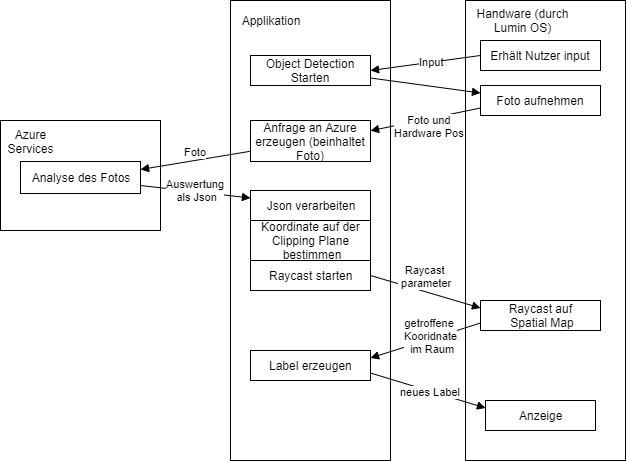
\includegraphics[width=1\textwidth]{images/dia_flow.png}
	\caption[]{Diagramm der Architektur inklusive Bearbeitungsschritte und Informationsweitergabe.}
	\label{dia:flow}
\end{figure}

% https://developer.magicleap.com/en-us/learn/guides/get-started-developing-in-unity
Das Projekt wurde in Unity umgesetzt und für die Magic Leap AR Brille entwickelt.
Es wurde ein Unity Projekt Template von Magic Leap verwendet. 

Zusätzlich werden einige vorgefertigte Klassen von Magic Leap verwendet. Dazu gehören MLInput, MLCamera, MLRaycast, MLPrivilegeRequestBehavior und MLSpatialMapper. Diese Klassen greifen auf Funktionalitäten des Lumin OS zu.

Die Benötigten Funktionalitäten der Applikation wurden in mehreren Script Klassen umgesetzt. Der Großteil der Scripts
 verhält sich wie Singletons. Sie existieren nur einmalig in der Szene.

Das Klassendiagramm auf Abbildung \ref{dia:classdiagramm} zeigt die Scripts und ihre Relationen zueinander.

\begin{figure}[H]
	\centering
	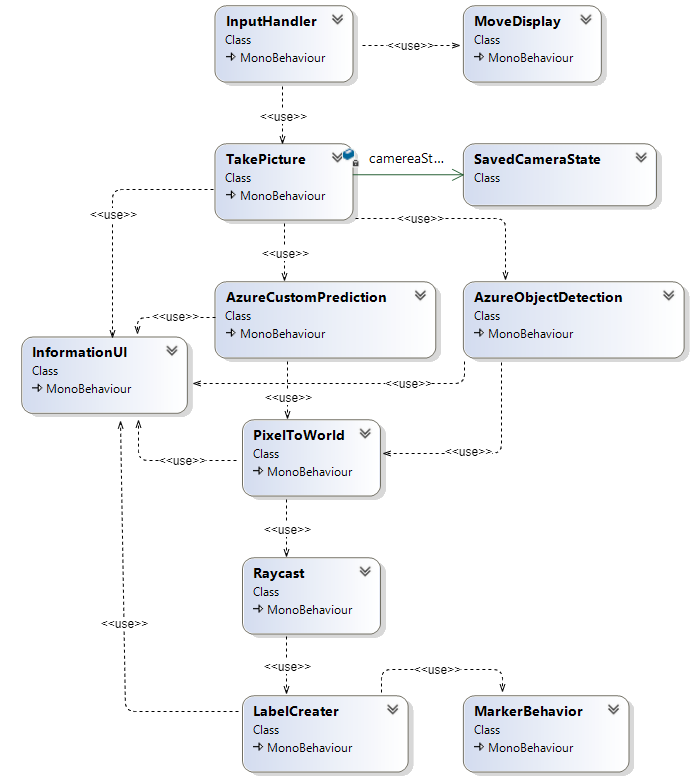
\includegraphics[width=1\textwidth]{images/klassendiagramm.png}
	\caption[]{Klassendiagramme der Scripte}
	\label{dia:classdiagramm}
\end{figure}
 
Die Klassen InputHandler, MoveDisplay, LabelCreater, InformationUI und MarkerBehavior sind für die Interaktion mit dem dem Nutzer zuständig. 

TakePicture, SavedCameraState, AzureCustomPredicton,AzureObjectDetection,PixelToWorld und Raycast führen das Erkennen von Labeln von Objekten anhand eines Aufgenommenen Fotos durch. Der Prozess wird duch den InputHander gestartet. 

Wurde ein Objekt erkannt und eine Position auf dem Mesh der Umgebung bestimmt, wird der LabelCreater aufgerufen. Es erzeugt das Label mit dem Entsprechenden Text.

MarkerBehavior ist eine Script das jedes Label GameObject hat, das erzeugt wird. Über das MarkerBehavior kann der Schriftzug des Labels angepasst werden.

\subsection{Interaktion}

InputHander verarbeitet den Input des Nutzers und startet entprechende Aktionen durch die MoveDisplay und TakePicture Klassen. 
MLInput ist eine vorgefertige Klasse von Magic Leap. Sie stellt Informationen über den Zustand des Controllers zur Verfügung. InputHander überwacht den Controller und startet die Aktionen, wenn die entsprechende Taste gedückt wurde.

\begin{itemize}
	\item Trigger: Objekt Erkennung starten mit TakePicture
	\item Home Button: UI Element Mittig vor das Display setzten.
	\item Bumper: Labels verstecken
	\item Bumper halten: zuletzt erzeugten Label entfernen 
\end{itemize}

Das UI Element wird von InformationUI gesteuert. TakePicture nutzt InformationUI um das zuletzt aufgenommene Foto anzuzeigen. AzureCustomPrediction, Azure ObjectDetection und PixelToWorld dokumentieren ihre Arbeitsschritte mit dem UI Element und der LabelCreater lässt eine Liste aller Labels anzeigen, die in der Szene existieren. Siehe Abbildung \ref{image:UIElement}.

%\begin{figure}[H]
%	\centering
%	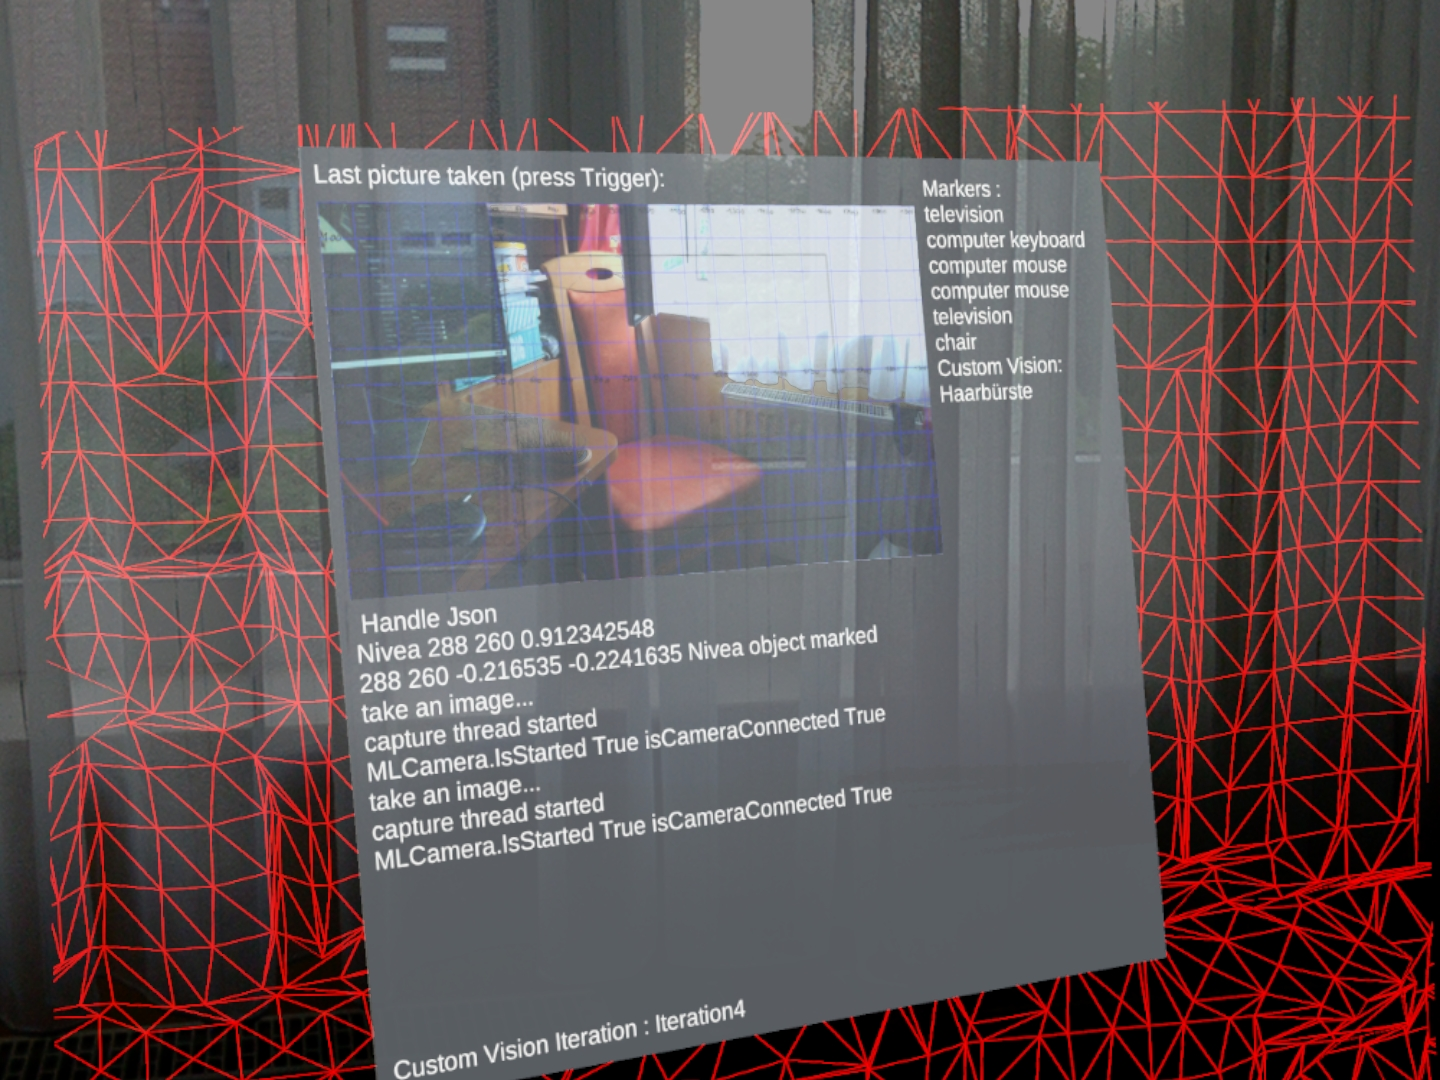
\includegraphics[width=1\textwidth]{images/ML_20200831_19.13.05.jpg}
%	\caption[]{UI Element}
%	\label{image:UIElement}
%\end{figure}

Der LabelCreater ist für das erstellen der Labels verantwortlich und sorgt dafür das die Labels für den Nutzer lesbar sind.
Dafür werden die Labels in Richtung der Kamera ausgerichtet und mitgeführt.
Des weiteren kann der LabelCreater Labels verstecken und entfernen.

Neben dem UI Element und den Labels wird auch ein Mesh angezeigt, das die Spatial Map der Umgebung wiedergibt. Das Spatial Mapping wird von Lumin OS durchgeführt und das Mesh wird durch die MLSpatialMapper Klasse von MagicLeap erzeugt.

\begin{figure}[H]
	\centering
	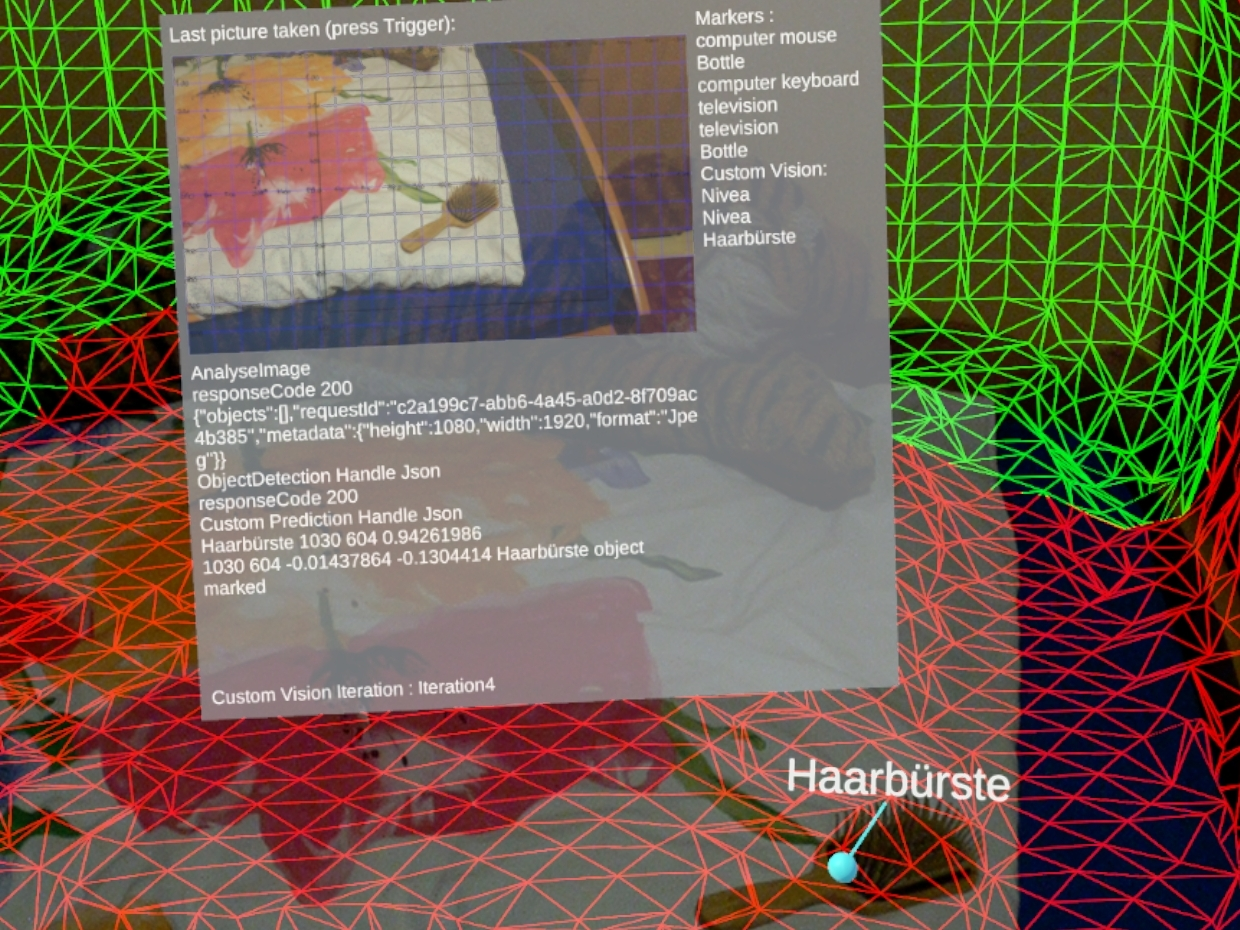
\includegraphics[width=0.9\textwidth]{images/ML_20201004_19.09.17_2.jpg}
	\caption[]{Ausgabe}
	\label{img:ausgabe}
\end{figure}


\subsection{Implementierung der Objekt Erkennung}

Im folgenden werden die Scripts besprochen die für die Objekt Erkennung zuständig sind.

\subsection{Ein Foto aufnehmen}

%\begin{figure}[H]
%	\centering
%	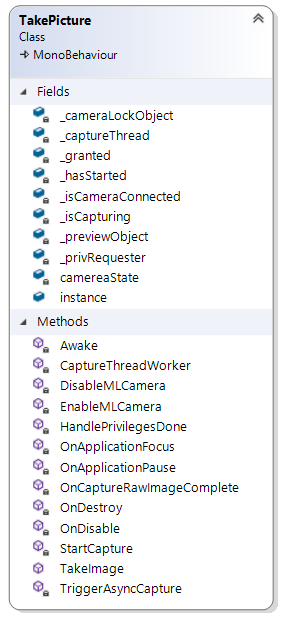
\includegraphics[width=0.4\textwidth]{images/dia_takepicture.PNG}
%	\caption[]{Klassendiagramm TakePicture}
%	\label{dia:takepicture}
%\end{figure} remake this image

Das Script TakePicture implementiert das Aufnehmen eines Fotos. Dabei wird MLCamera von MagicLeap genutzt, um die Kamera der Magic Leap Brille anzusteuern. Wenn die Applikation gestartet wird, stellt dieses Script sicher, das Applikation Permission hat die Kamera zu nutzen. Dannach verbindet sich das Script über MLKamera mit der Kamera Ressource. 
Die Kamera Ressouce wird wieder abgegeben, wenn die Appliaktion terminiert oder pausiert wird.

Wenn die Methode TakeImage aufgerufen wird, startet der Prozess der Objekt Erkennung.
Das aufnehmen der Fotos geschieht asynchron. Für jedes Foto wird ein Thread erzeugt, in dem MLCamera ein Foto aufnimmt. In diesem Thread wird zusätzlich die Aktuelle Position der Unity Kamera als SavedCameraState gespeichert.

Die Methode OnCaptureRawImageComplete wird von MLCamera aufgerufen, wenn das Foto fertig ist. Die Daten des Bildes und der SavedCameraState werden von dort aus an die Scripts AzureObjectDetection und AzureCustomPrediction weitergegeben. Dort wird die Analyse der Bilder gestartet. 

\subsubsection{Object Detection}

\begin{figure}[H]
	\centering
	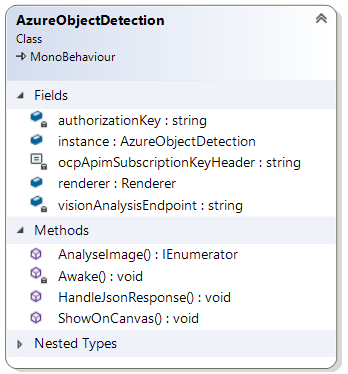
\includegraphics[width=0.5\textwidth]{images/dia_azureobjectdetection.PNG}
	\caption[]{Klassendiagramm AzureObjectDetection}
	\label{dia:azureobjectdetection}
\end{figure}

In der Methode AnalyseImage von AzureObjectDetection wird ein Web Request zusammengestellt, um die Azure REST API anzufragen. Der Request enthält einen Authentifizierung für die API und das zu analysierende Foto. %Siehe Abbildung \ref{dia:azureobjectdetection}.

Der Webrequest wird verschickt und auf die Antwort gewartet. Wenn die Antwort eintrifft, wird anhand des ResponseCodes geprüft, ob es bei dem Request einen Fehler gab. Beispielsweise kann die Internetverbindung gestört sein oder die Authentifizierung abgelehnt werden.
Wenn es keinen Fehler gab, wurde eine Json-Datei bei der Antwort mitgeschickt. Darin wird für jedes gefundene Objekt auf dem Foto eine Bezeichnung (Klasse) und eine Bounding Box angegeben. 

Die Json-Datei wird in HandleJsonResponse verarbeitet. Für den erwarteten Aufbau der Datei wurden drei Klassen geschrieben. Der Json String wird mit JsonUtility in ein DetectionResponse Object umgewandelt. Dabei werden alle gefundenen Foto-Objekte in einer Liste von DetectedObjects abgelegt. Siehe Abbildung \ref{dia:jsonClasses}. \citep{fromjson}

\begin{figure}[H]
	\centering
	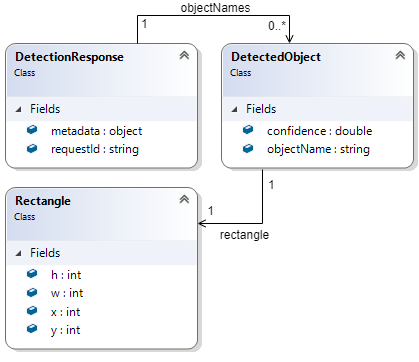
\includegraphics[width=0.6\textwidth]{images/dia_json.PNG}
	\caption[]{Umwandeln der Json Datei in Objekte.}
	\label{dia:jsonClasses}
\end{figure}

Die gefundenen Objekte sollen im 3D Raum mit einem Label gekennzeichnet werden. 
Dafür wird für jedes DetectedObject die Methode Cast von der Klasse PixelToWorld aufgerufen. Der Methode wird der Mittelpunkt der BoundingBox als u,v Foto-Koordinate für das DetectedObject übergeben. Siehe Abbildung \ref{code:handlejson}.

\begin{figure}[H]
	\centering
	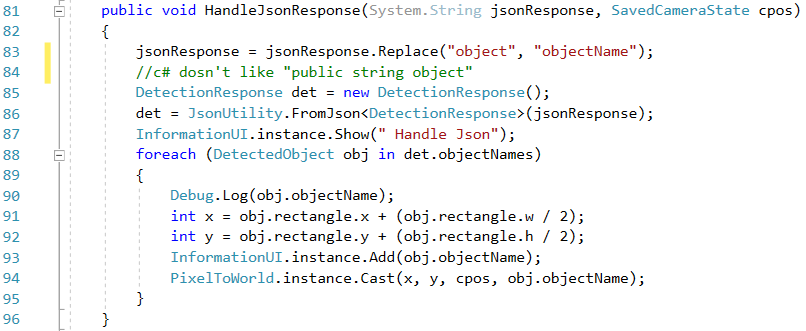
\includegraphics[width=1\textwidth]{images/code_handleJson.PNG}
	\caption[]{Umwandeln der Json Datei in Objekte.}
	\label{code:handlejson}
\end{figure}

\subsubsection{Von dem Foto zum 3D Raum}

\begin{figure}[H]
	\centering
	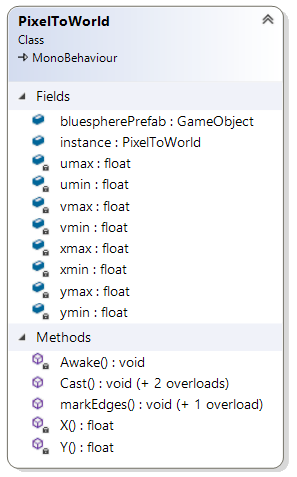
\includegraphics[width=0.45\textwidth]{images/dia_pixeltoworld.PNG}
	\caption[]{Klassendiagramm PixelToWorld}
	\label{dia:pixeltoworld}
\end{figure}

Ein gefundenes Foto-Objekt soll in der 3D Abbildung der realen Welt lokalisiert werden. Dafür nutzt die Methode Cast die u,v Foto-Koordinate des Objekts und einen SavedCameraState. Der SavedCameraState beschreibt die Positiong der Unity Kamera zu dem Zeitpunkt als das Foto aufgenommen wurde. SavedCameraState beinhaltete die cameraToWorldMatrix und den Urspung der Kamera.

Das Foto kann mit dem Display und somit mit der Clipping Plane der Hauptkamera approximiert werden.
Die u,v Foto-Koordinate wird zunächst in eine x,y,z Koordinate in dem Camera Space umgewandelt. Der z Anteil gibt die Entfernung von dem Ursprung der Kamera an in Blickrichtung an. Dabei befinden sich Punkte mit einer Entfernung von 0.4 Einheiten auf der Clipping Plane. In dem Camera Space mit z = -0.4 angegeben. 

Die x und y Dimensionen beschreiben die Achsen, die horizontal und vertikal zur Clipping Plane verlaufen. Mit dem festgelegten z = -0.4, kann jeder Punkt auf der Clipping Plane durch x und y angegeben werden. Dazu gehören auch Punkte die außerhalb des View Frustum liegen.

Es wurden Werte für x und y ausprobiert, mit denen die Ränder des Fotos auf der Clipping Plane angegeben werden können. Dabei wurde auf die unterschiedlichen Seitenverhältnisse des Fotos und des Displays geachtet. Darüber hinaus ist der Bildausschnitt des Displays kleiner. Daher liegen die Ränder des Fotos außerhalb des View Frustum. 

Sind diese x und y Werte bekannt, ergibt sich für die Achsen jeweils ein Intervall, die kombiniert alle Foto-Koordinaten auf die Clipping Plane abbilden können. Die Intervall lauten: [-0.295,0.2281] für x und [0.1546,-0.1507] für y. Mit den Intervallen wird die Position und Skalierung des Fotos in Relation zu dem Display - und der Hauptkamera - berücksichtigt. Siehe Kapitel \ref{section:devpixeltoworld} für die Entwickelung der Cast Methode und die Ermittlung der Intervallwerte.

Es werden zwei lineare Funktionen aufgestellt:
\begin{itemize}
	\item Die Funktion X bildet das Intervall für u [0,1920] auf das Intervall für x [-0.295,0.2281] ab.
	\item Die Funktion Y bildet das Intervall für v [0,1080] auf das Intervall für y [0.1546,-0.1507] ab.
\end{itemize}
Siehe Abbildung \ref{code:uvtoxy}.
\begin{figure}[H]
	\centering
	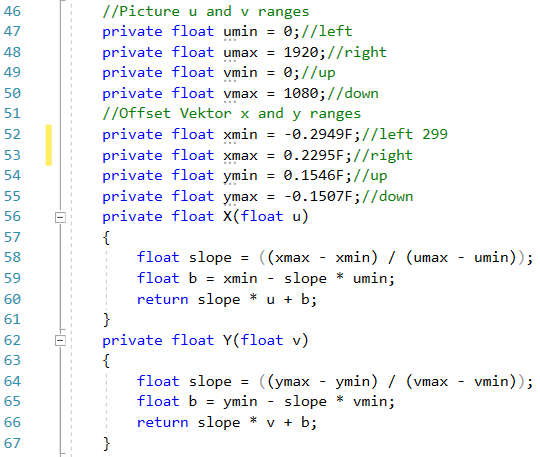
\includegraphics[width=0.6\textwidth]{images/code_uv_to_xy_scale.PNG}
	\caption[]{Funktionen X und Y}
	\label{code:uvtoxy}
\end{figure}

Mit den Funktionen wird eine Koordinate im Camera Space für u,v berechnet. Diese Koordinate wird dann, mithilfe der cameraToWorldMatrix des SavedCameraState, in die Koordinate p des globale Koordinatensystem umgewandelt. Damit wird die Position und Rotation der Kamera - und somit des Fotos - in der 3D Szene berücksichtigt. Siehe Abbildung \ref{code:castmethod}.

\begin{figure}[H]
	\centering
	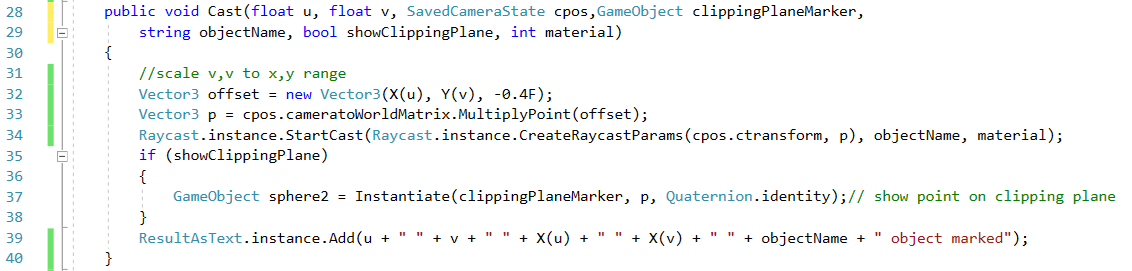
\includegraphics[width=1.2\textwidth]{images/code_cast_method.PNG}
	\caption[]{Cast Methode}
	\label{code:castmethod}
\end{figure}
\subsubsection{Raycast}

\begin{figure}[H]
	\centering
	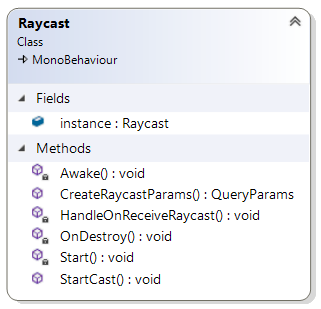
\includegraphics[width=0.45\textwidth]{images/dia_raycast.PNG}
	\caption[]{Klassendiagramm Raycast}
	\label{dia:raycast}
\end{figure}

Als Nächstes wird ein Raycast durch den Ursprung der Kamera und die Koordinate p gesendet. MLRaycast wird genutzt, um einen Schnittpunkt mit der Rekonstitution der Welt von Lumin OS zu bestimmen. Die Stelle, die der Raycast trifft beschreibt die Position des DetectedObject im 3D Raum.

Für den MLRaycast werden zwei Parameter benötigt:
\begin{itemize}
	\item Ein QueryParams Objekt, das Ursprung und Richtung für den Raycast beinhaltet.
	\begin{itemize}
		\item Ursprung: Kameraursprung aus SavedCameraState
		\item Richtung: Richtungsvektor von dem Kameraursprung zu der Koordinate p
	\end{itemize}
	\item Eine Methode die aufgerufen wird, wenn der Raycast fertig ist. 
	\begin{itemize}
		\item Callback Methode: HandleOnRecieveRaycast
	\end{itemize}
\end{itemize}

Siehe Abbildung \ref{code:raycastparams}.

\begin{figure}[H]
	\centering
	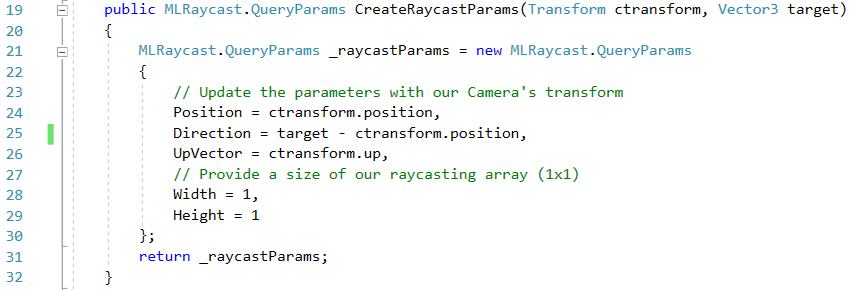
\includegraphics[width=1\textwidth]{images/code_raycastparams.PNG}
	\caption[]{Cast Methode}
	\label{code:raycastparams}
\end{figure}

Wenn der Raycast fertig ist, wird die Methode HandleOnRecieveRaycast aufgerufen. Der Parameter point beinhaltet dabei die getroffene Koordinate.
Diese wird an die Methode CreateMarker von der Klasse LabelCreater weitergegeben.

\subsubsection{LabelCreater}

\begin{figure}
	\centering
	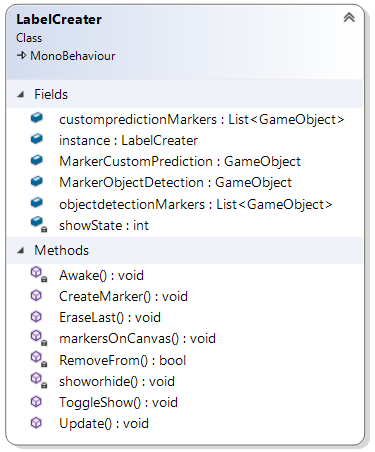
\includegraphics[width=0.5\textwidth]{images/dia_labelcreater.PNG}
	\caption[]{Markierungen in der Welt}
	\label{dia:labelcreater}
\end{figure}

CreateMarker erhält den Punkt point, der getroffen wurde und die Bezeichnung für das DetectedObject. An der Koordinate von point wird ein Prefab GameObject instanziiert, das als Markierung für das DetectedObject in der 3D Umgebung dient.

Das Prefab besteht aus einer Kugel und einem Schriftzug, der den Namen des DetectedObject anzeigen soll. Dem neu instanziierten GameObject wird die Bezeichnung des DetectedObject als Schriftzug zugewiesen. Siehe Abbildung \ref{image:labels}.

\begin{figure}[H]
	\centering
	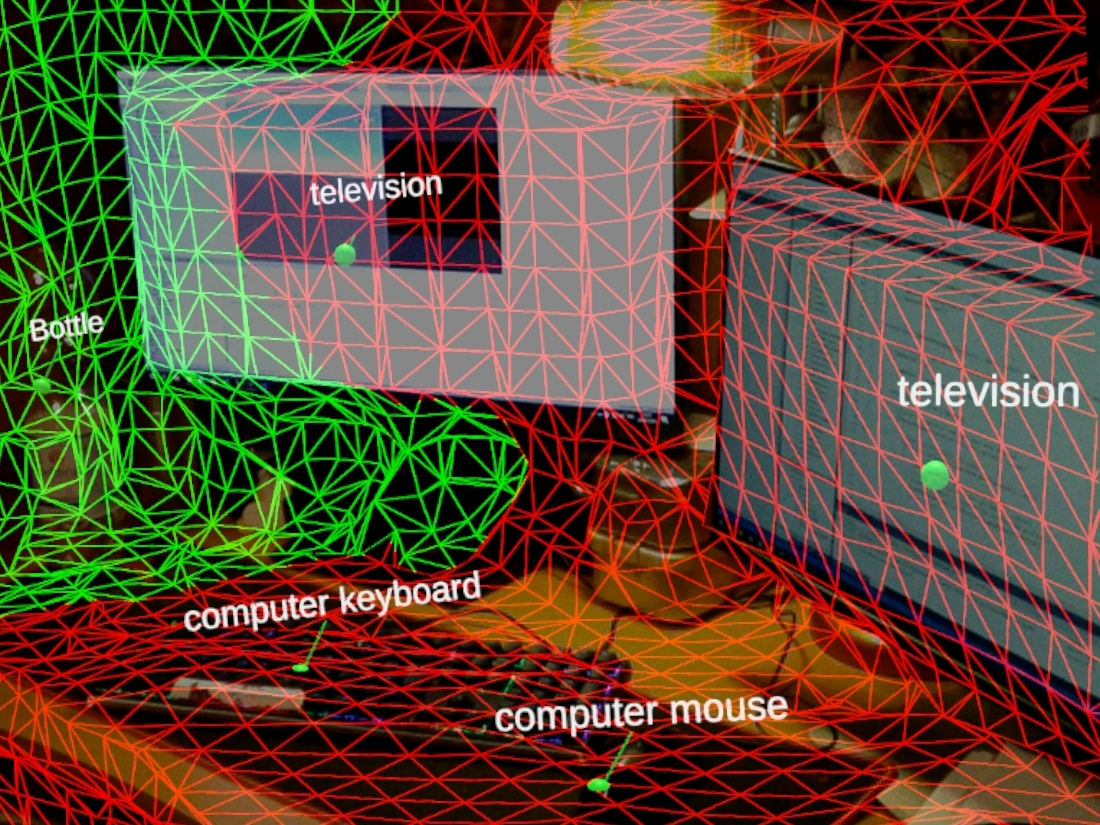
\includegraphics[width=0.8\textwidth]{images/ML_20201004_19.10.05_2.jpg}
	\caption[]{Labels in der Welt}
	\label{image:labels}
\end{figure}

Wenn ein Label nahe eines anderen Labels erzeugt werden soll, das denselben Schriftzug hat, wird davon ausgegangen, das ein Objekt der Realen Welt zum zweiten mal erkannt wurde. Daher wird kein neues Label erstellt, sondern das alte Label modifiziert.
Die Positionen an denen das Objekt in der Szene lokalisiert wurde werden mit jeweils einer grauen Sphäre markiert und das Label wird in den Mittelpunkt der grauen Sphären gesetzt.
So  wird die Position des Objektes genauer, wenn es häufiger Erkannt wurde. Siehe Abbildungen \ref{image:multi1} und \ref{image:multi2}.

\begin{figure}[H]
	\centering
	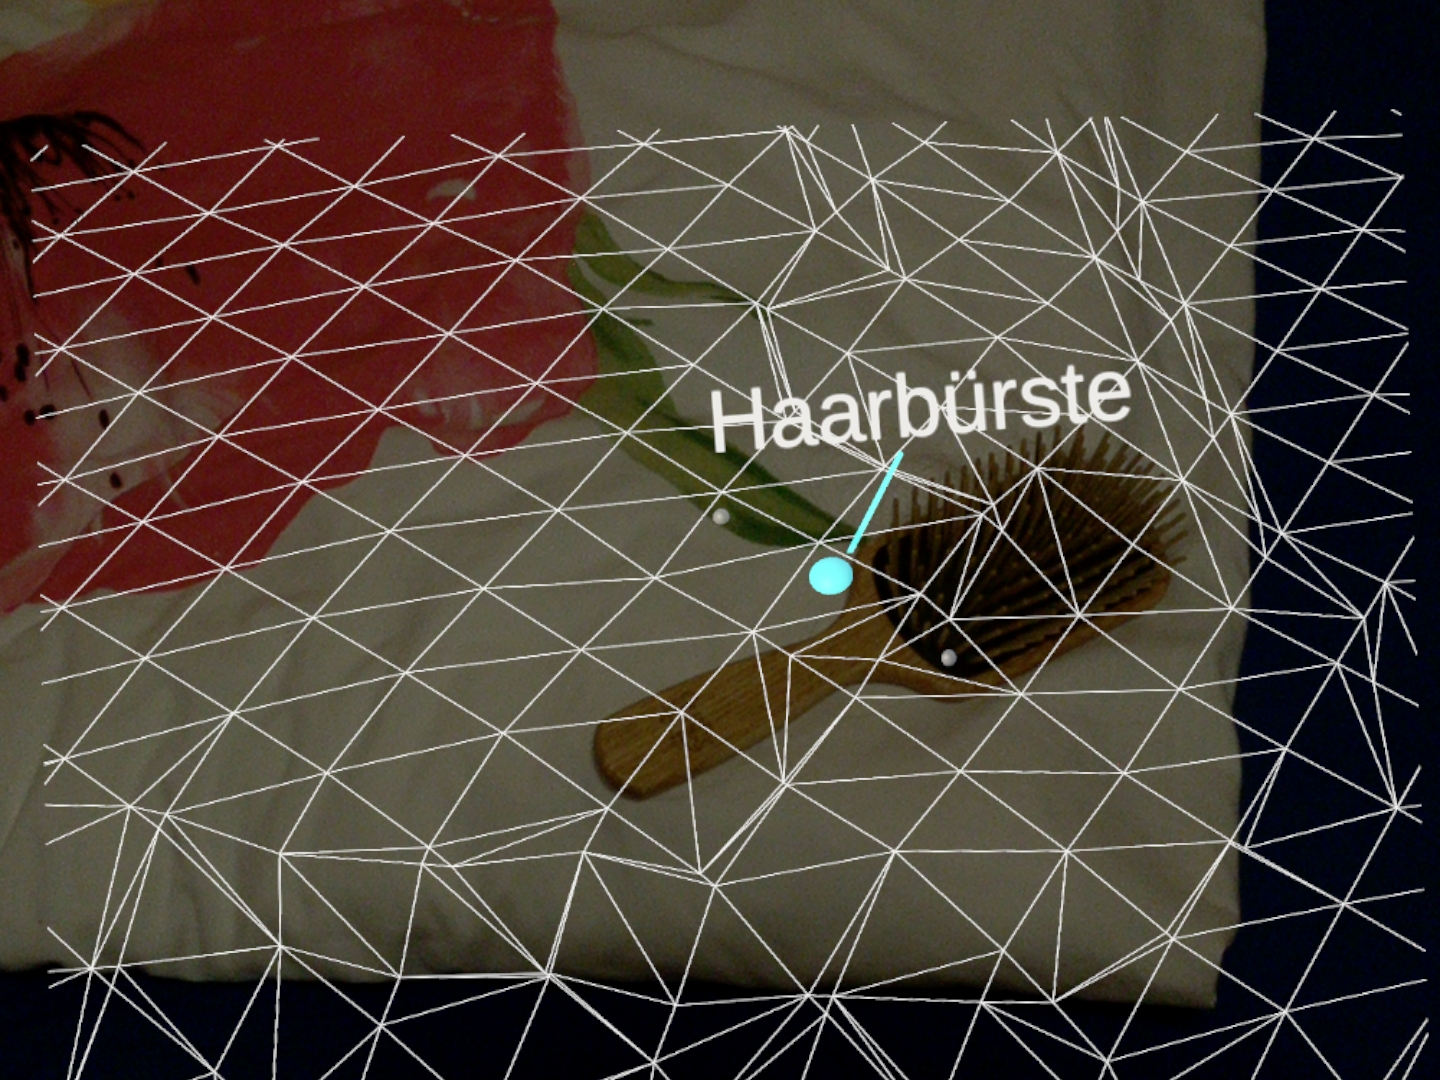
\includegraphics[width=0.7\textwidth]{images/ML_20201004_19.12.40.jpg}
	\caption[]{Haarbürste zwei mal Erkannt}
	\label{image:multi1}
\end{figure}


\begin{figure}[H]
	\centering
	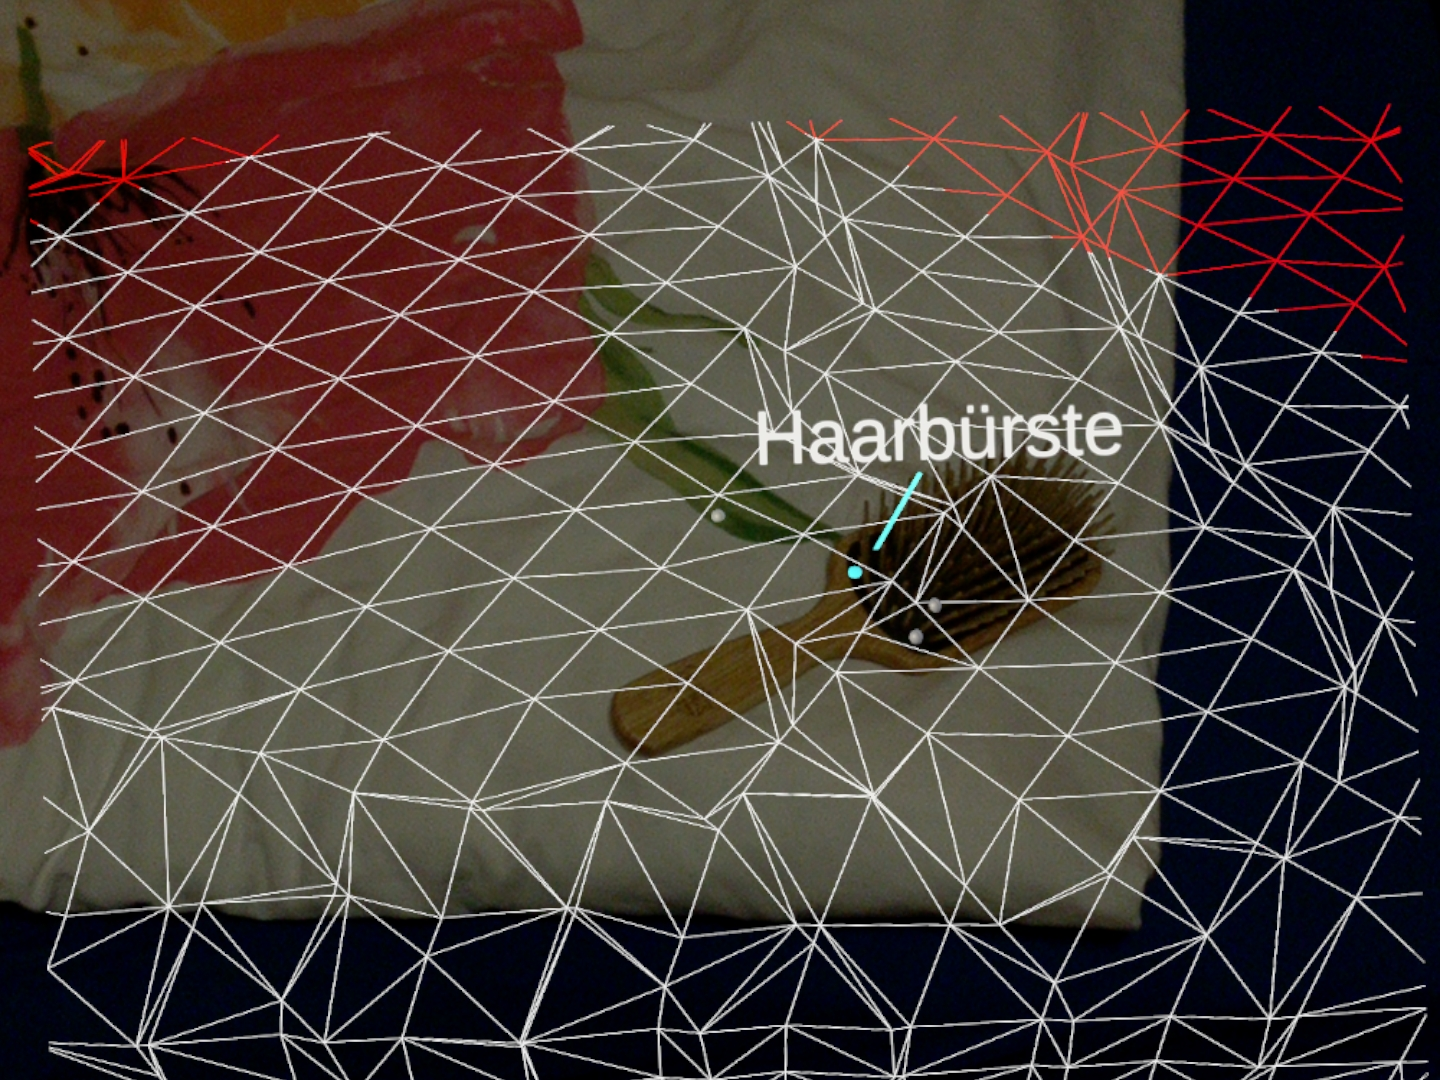
\includegraphics[width=0.7\textwidth]{images/ML_20201004_19.13.07.jpg}
	\caption[]{Haarbürste drei mal Erkannt}
	\label{image:multi2}
\end{figure}


Die erzeugten Labels werden in den Listen MarkerCustomPredicton und MarkeroBjectDetection gespeichert, je nachdem welcher Azrue Service verwendet wurde. 
Die Listen werden genutzt, um die Labels zu der Unity Kamera auszurichten damit sie lesbar sind. 

\subsubsection{Azure Custom Vision}

Neben der Bildanalyse mit Azure Object Detection wird auch Azure Custom Vision verwendet.
Die AI wurde über die Webseite trainiert.

Die Anfrage an den Service passiert in der Klasse AzureCustomPrediction. Ähnlich wie bei AzureObjectDetection wird ein Webrequest erstellt mit einem Authorization Key für den Service und einem Foto als Payload.

In der Antwort wird eine Json Datei zurückgeschickt, die die gefundenen Objekte angibt.
Da die Json Datei eine etwas anderes Format hat, wurde eine eigene HandleJsonResponse Methode dafür geschrieben.

Für jedes erkannte Objekt wird die Methode Cast von PixelToWorld aufgerufen, um das Objekt in der realen Welt zu lokalisieren und zu markieren.

\paragraph{Das Trainieren}

Es wurde probiert das Custom Vision Modell auf drei unterschiedliche Objekte zu trainieren.
Dabei wurden vier Iterationen erstellt. 

Iteration 1:

Zunächst wurde probiert Tuben von Acrylfarbe zu erkennen. Die Genauigkeit davon war nicht sehr hoch. Es wurden in Fotos Acrylfarben an Stellen erkannt, an denen es keine gab. Siehe Abbildung \ref{image:customVisionPaint}. 

\begin{figure}[H]
	\centering
	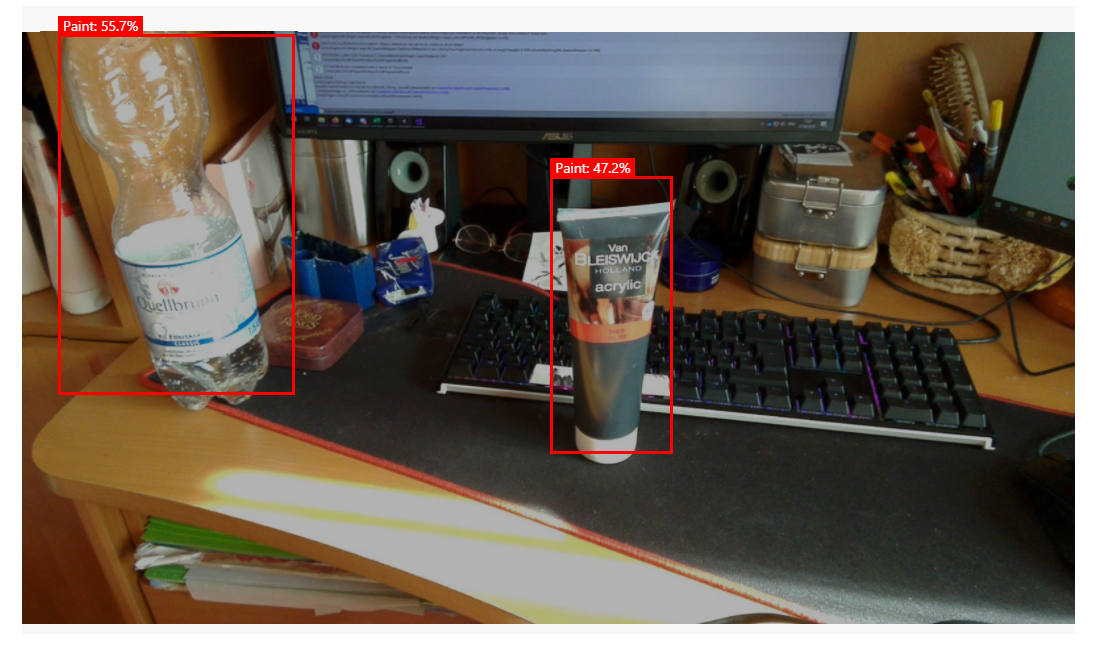
\includegraphics[width=1.0\textwidth]{images/customVisionPaint.PNG}
	\caption[]{Beispielfoto Iteration 1. Die Wasserflasche wurde als Farbe markiert mit 55.7 Prozent statistischer Konfidenz. Die Tatsächliche Farbtube wurde mit einer Konfidenz von 47.5 Prozent erkannt.}
	\label{image:customVisionPaint}
\end{figure}

\paragraph{Iteration 2}

In der zweiten Iteration wurde probiert das Modell darauf zu trainieren, eine blaue Dose von Nivea Hautcreme to erkennen. Die Form und Farbe der Dose ist sehr simpel, daher wurde davon ausgegangen, dass sie leichter zu erkennen ist. Die berechnete Prediction Wahrscheinlichkeit während des Trainings lag bei 80 Prozent.

Trotzdem wurden in vielen Fotos fälschlicherweise Nivea Dosen erkannt. 

\paragraph{Iteration 3}

In der dritten Iteration wurde versucht die vorherige Iteration zu verbessern. Es wurden ausgewählte Trainingsfotos entfernt, die die Dose von einem seitlichen Winkel zeigten. Die Erwartung war, dass die Detektion der Dose aus dem Blickwinkel von Oben konsistenter wird. Zusätzlich wurden mehr Fotos von der Dose auf unterschiedlich gefärbten und gemusterten Untergründen hinzugefügt. 

Die Genauigkeit der Prediction sank auf 75 Prozent.

\paragraph{Iteration 4}

In der vierten Iteration wurden zwei Fotos von der Nivea Dose entfernt, was die Genauigkeit auf 100 Prozent steigen ließ. In der Umsetzung mit der Magic Leap Anwendung wurden trotzdem häufig Objekte fälschlicherweise als Nivea Dose markiert.

Neben der Dose wurde diese Iteration darauf trainiert eine bestimmte Holzhaarbürste zu erkennen. Aufgrund von dem komplexeren, und markanten Aussehen der Bürste wurde davon ausgegangen, das die Bürste besser von anderen Objekte zu unterschieden ist. 
Die Bürste wurde nur mit den Borsten nach oben fotografiert.

Die Genauigkeit für die Bürste lag bei 100 Prozent. 
In der Umsetzung mit der Magic Leap Anwendung wird die Bürste häufig nicht erkannt, obwohl sie im Bild ist und mit den Borsten nach oben liegt. Es werden jedoch keine Objekte fälschlicherweise als Haarbürste erkannt.

\subsection{Entwicklung der Foto-Repräsentation}
\label{section:devpixeltoworld}

Um die u,v Foto-Koordinate eines gefundenen Objektes auf der Clipping Plane der Kamera zu lokalisieren, wurden ein paar Herangehensweisen ausprobiert.

Das Ziel ist das Setzten einer Markierung in dem 3D Raum, basierend auf der Foto-Koordinate. Das Foto beinhaltet keine Information über die Entfernung zu dem Objekt. Dafür muss ein Raycast durchgeführt werden. 

Mit einer Repräsentation des Fotos in dem 3D Raum ist es möglich diesen Raycast durchzuführen. 
Dazu muss das Foto nicht tatsächlich in dem 3D Raum vorhanden sein. Es muss jedoch mit dem Input einer Foto-Koordinate ein Output einer Koordinate in dem 3D Raum erzeugt werden, mit dem der Raycast durchgeführt werden kann.

Die Position des Fotos hängt mit der Kamera zusammen, daher kann das Foto durch den Camera Space simuliert werden. Als erstes wurde probiert ein Sphären-Objekt an eine gezielte Koordinate des Camera Space zu bewegen. 

% make pretty after this
Wenn die Kamera am Ursprung des globalen Koordinatensystem liegt und eine neutrale Rotation hat, stimmt der Camera Space mit dem globalen Koordinatensystem überein. Die Sphäre wurde in der Szene per Hand bewegt um markante Koordinaten des Camera Space abzulesen. Siehe Abbildung \ref{illustration:speretest}.

\begin{figure}[H]
	\centering
	\includegraphics[width=0.7\textwidth]{images/sphärenTest.PNG}
	\caption[]{Die Blaue Sphäre liegt auf dem Rechten Rand der Clipping Plane.}
	\label{illustration:speretest}
\end{figure}

Dabei wurden folgende Camera Space Koordinaten gefunden:
\begin{itemize}
	\item Near Clipping Plane bei z = -0.37
	\item linker Rand bei x = -0.153
	\item rechter Rand bei x = 0.153
	\item oberer Rand bei y = 0.1147
	\item unterer Rand bei y = -0.1147
\end{itemize}

Die x und y Koordinaten hängen von der u,v Koordinate des Fotos ab. Es wurden lineare Funktionen aufgestellt um u,v auf x,y abzubilden. Diese Abbildung dient als Repräsentation des Fotos im 3D Raum, unter Berücksichtigung der Position und Skalierung des Fotos im Verhältnis zu der Kamera.

Dann wurde getestet wie genau DetectedObjects in der AR Umgebung lokalisiert werden. Es wurden testweise Fotos aufgenommen, analysiert und die DetectedObjects markiert. Die entstandenen Markierungen lagen in Sichtfeld, jedoch nicht an den erwarteten Stellen. 

Um dem Problem auf den Grund zu gehen, wurde ein UI Objekt erstellt, das ein aufgenommenes Foto bei Runtime anzeigt.
Das Foto wurde dann mit dem Display verglichen. Dabei fiel auf, das sie ein unterschiedliches Seitenverhältnis haben und das Display einen kleinen Bildausschnitt zeigt.  

Es gibt zwei Möglichkeiten die Unterschiede zwischen Foto und Display auszugleichen. Entweder wird das Foto auf das Display zugeschnitten oder das gesamte Foto wird verwendet. Im zweiten Fall würden auch Objekte erkannt, die außerhalb des Sichtfeldes liegen.
Es wurde die Entscheidung getroffen das Foto zuzuschneiden. Damit gibt es ein besseres Feedback für den Nutzer, wenn ein Objekt gefunden wurde. 

Das Zuschneiden wurde realisiert, indem die Intervalle für u und v der Abbildungsfunktionen stärker eingegrenzt wurden. Alle Objekte die außerhalb der Intervalle liegen werden ignoriert. Um die Intervalle zu bestimmen wurde dem Fotoanzeige-UI-Element ein Gitter hinzugefügt. Mit dem Gitter kann die u,v Position von beliebigen Stellen des Fotos abgelesen werden. 
Durch Aufnehmen von Fotos und Vergleichen mit dem Sichtfeld des Displays wurde abgelesen, bei welcher u,v Position des Fotos die Ecken des Displays zu finden sind. Die Intervalle wurden dem entsprechend eingegrenzt. 

Mit den durchführten Veränderungen der Intervalle konnten DetectedObjects korrekt in der Umgebung lokalisiert werden. Jedoch wurden sehr häufig Objekte nicht markiert, obwohl sie im Sichtfeld des Nutzers lagen, weil deren Mittelpunkt außerhalb eines Intervalls lag.

Daher wurde entschieden die zweite Möglichkeit zu implementieren und das gesamte Foto zu verwenden und Objekte auch zu markieren, wenn sie komplett außerhalb des Sichtfeldes liegen. 
Dafür wurden die Intervalle für u und v wieder auf die ursprünglichen Werte - [0,1920] und [0,1080] - gesetzt. Die Intervalle für x und y mussten vergrößert werden.

Um die x und y Intervalle bestimmen zu können, wurde das Fotoanzeige-UI-Element Parallel zu der ClippingPlane gelegt. Das Element folgt den Bewegungen der Kamera und liegt möglichst nah an der Near Clipping Plane. Das Display der Magic Leap Brille zeigt selbst solide Objekte leicht durchsichtig an. Das wurde genutzt, um Fotos aufzunehmen, mit dem UI Element anzuzeigen und mit der realen Welt zu vergleichen. Durch Ausprobieren wurde das UI Element so skaliert und verschoben, dass das angezeigte Foto mit der realen Welt soweit wie möglich übereinstimmt. Siehe Abbildungen \ref{illustration:canvasinsourface} und \ref{illustration:canvasinsourfacetodown}.

\begin{figure}[H]
	\centering
	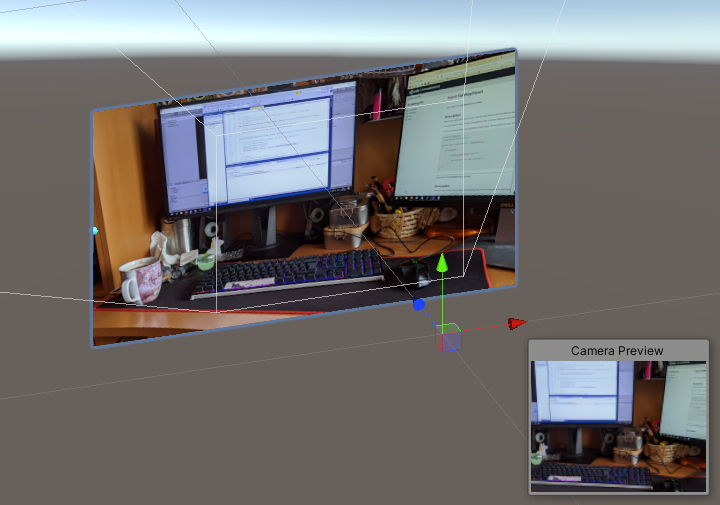
\includegraphics[width=0.7\textwidth]{images/canvasinyourface.PNG}
	\caption[]{Das Aufgenommene Foto füllt das gesamte Display aus, wenn es angezeigt wird. Die Blaue Sphäre liegt auf dem Rechten Rand des Foto-Anzeige-Elementes.}
	\label{illustration:canvasinsourface}
\end{figure}

\begin{figure}[H]
	\centering
	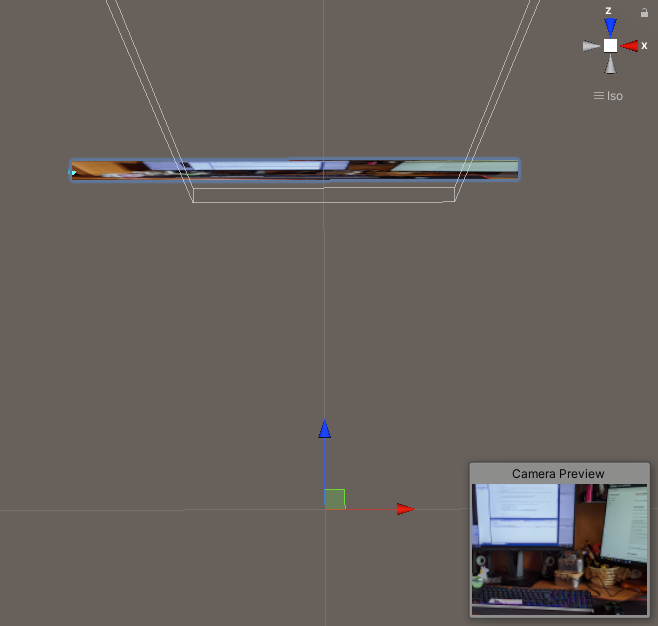
\includegraphics[width=0.7\textwidth]{images/canvasinyourfaceTopDown.PNG}
	\caption[]{Die Blaue Sphäre befindet sich nicht mehr in dem View Frustum und das Foto-Anzeige-Element befindet sich ein wenig hinter der Near Clipping Plane.}
	\label{illustration:canvasinsourfacetodown}
\end{figure}

Dann wurden die Ränder des UI Elementes genutzt um die Intervalle für x und y zu bestimmen.
\begin{itemize}
	\item für x: [-0.295, 0.2281]
	\item für y: [0.1546, -0.1507]
	\item Zusätzlich wurde z = -0.4 gesetzt. Das UI Element musste ein wenig weiter von der Clipping Plane entfernt sein um angezeigt zu werden.
\end{itemize}

Mit diesen Intervallen für u,v,x und y konnten DetectedObjects gut lokalisiert werden und es wurden keine Objekte mehr weggelassen, von denen der Nutzer erwarten würden, das sie markiert werden.

\newpage
\section{Auswertung}

in welchem raum getestet. wie groß sind die fotos?

\subsection{Laufzeitanalyse}

Die Laufzeit von dem Aufnehmen und Analysieren eines Fotos bis hin zur Label Erstellung in der Szene wurde aufgezeichnet. Siehe Abbildung \ref{img:laufzeit}

\begin{figure}[H]
	\centering
	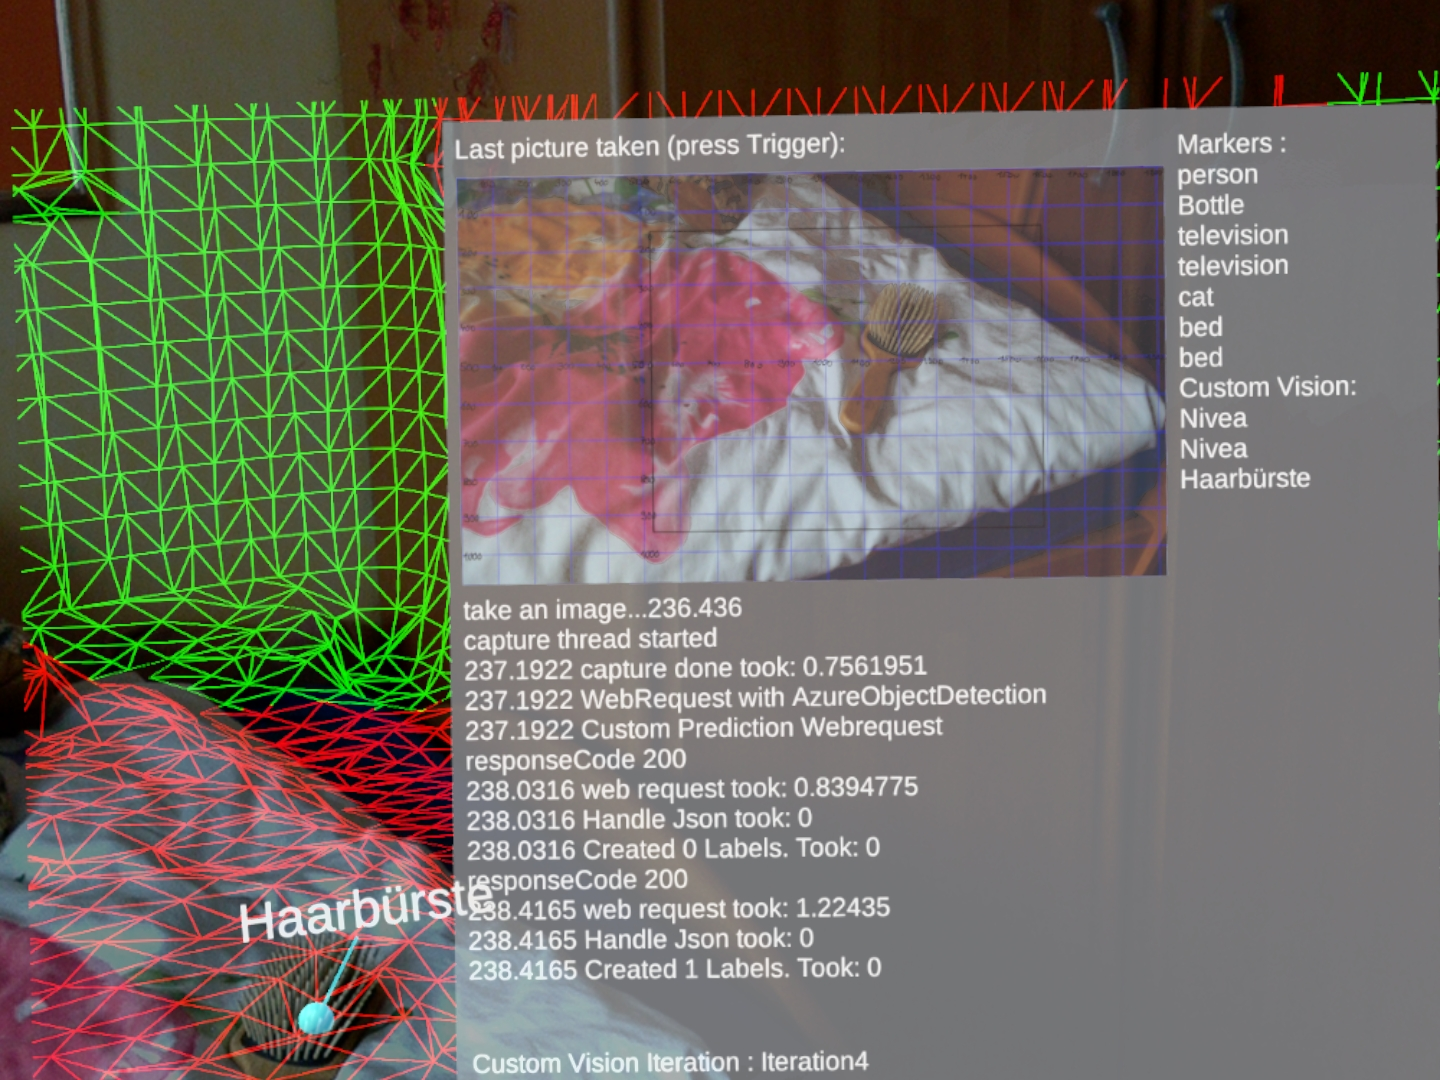
\includegraphics[width=0.9\textwidth]{images/ML_20201005_16.12.36.jpg}
	\caption[]{Durchlauf mit Laufzeit Aufzeichung}
	\label{img:laufzeit}
\end{figure}

Über 11 Aufgenommene Fotos wurden gefunden, das das Aufnehmen des Fotos im Durchschnitt 0,9 Sekunden dauert. Das Anfragen des Azure Object Detection Services, inklusive Netzwerk Response Time liebt durchschnittlich bei 1,01 Sekunden. Die Anfrage an den Azure Custom Vision Service, inklusive Netzwerk Response Time, dauert im durchschnitt 1,28 Sekunden. 

Das auslesen der Json Antworten, lokalisieren der Objekten in der 3D Szene und das Label erstellen, benötigt weniger als eine Mikrosekunde.

Insgesamt dauert das Aufnehmen und Analysieren eines Fotos somit durchschnittlich 3,19 Sekunden. Siehe Abbildung \ref{table:laufzeitanalyse} und \ref{table:laufzeitanalyse2}.

\begin{figure}[H]
	\centering
	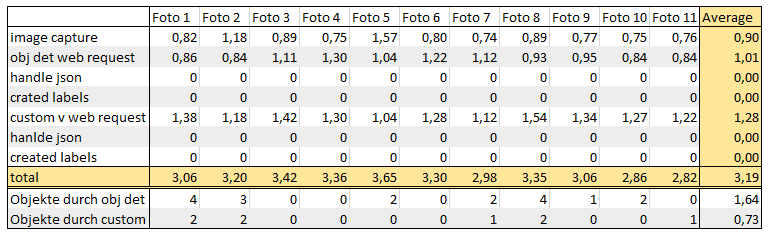
\includegraphics[width=1\textwidth]{images/table_Laufzeitanalyse.PNG}
	\caption[]{Laufzeitanalyse über 11 Bild-Analysen.}
	\label{table:laufzeitanalyse}
\end{figure}

\begin{figure}[H]
	\centering
	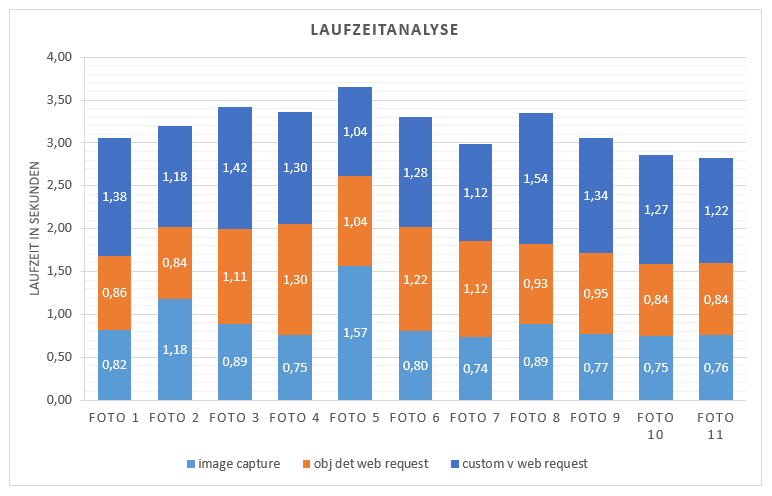
\includegraphics[width=0.9\textwidth]{images/table_Laufzeitanalyse2.PNG}
	\caption[]{Diagramm Laufzeitanalyse}
	\label{table:laufzeitanalyse2}
\end{figure}

Gedanken dazu: Für die Laufzeit ist es besser ein einziges Network zu nehmen. Und das Image Capture so lange dauert ist eigenldich unacceptable. Das sollte schneller gehen. Dadurch statt einzelne Fotos aufzunehmen ein contiousouls video aufnehmen und frames davon zu analysieren wäre besser. Ist auf jeden Fall nicht real time.

Durchschnittlich wurden durch Objekt Detection 1.64 Objekte pro bild erkannt und durch custom detection 0.73.

\subsection{Analyse durch Azure Objekt Detection}

Wie sieht der raum aus?
Welche objekte wurden erkannt. 
Wie wurden sie misinterpretet.
Objekte erkennen auch wenn sie nicht komplett im screen sind.

\subsection{Azure Custom Vision}

kommt halt darauf an wie es trainiert ist. 

\subsection{Objekte in 3D Szene Lokalisieren}

generell gut. Durch mehrere detectionen wird lokation verbessert, besonders wenn durch leicht unterschiedliche Blickwinkel. Aber auch bei nur einer Erkennung ist die Position in der 3D Szene ganz gut. 

%todo

spatial mapping braucht manchmal ne weilse, das dazu führt, das das label nicht an der richtigen stelle ist.
passiert bei objekten die sich oft bewegen, wie ein stuhl. Siehe Abbildung \ref{img:stuhl}.
\begin{figure}[H]
	\centering
	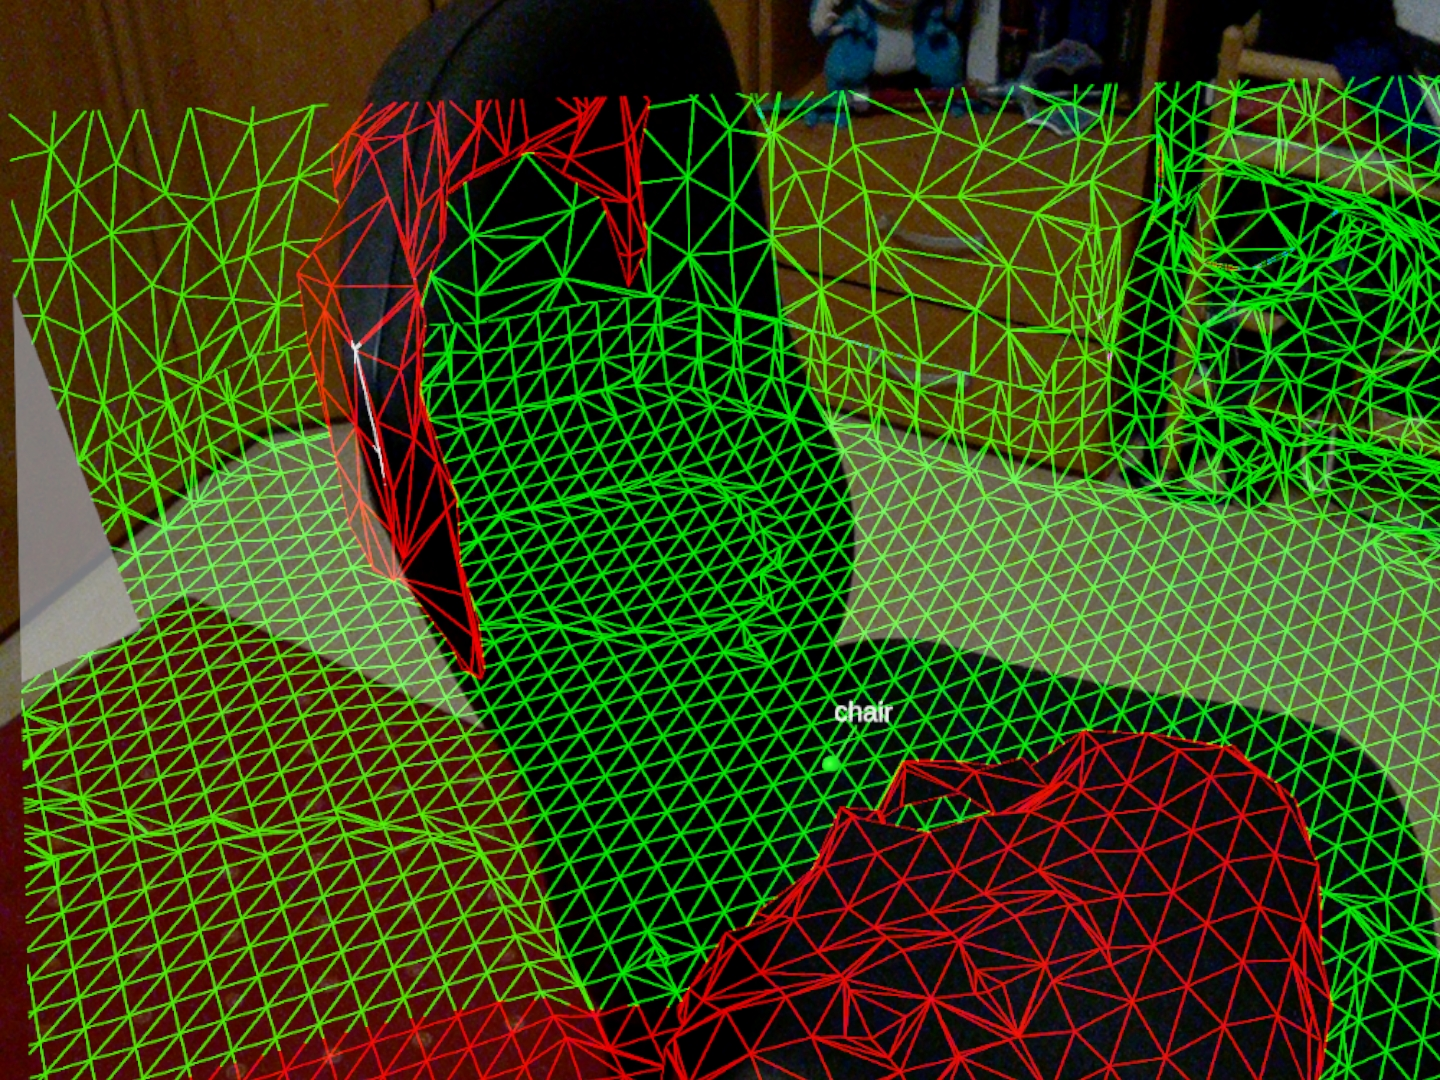
\includegraphics[width=0.8\textwidth]{images/ML_20201004_19.18.02.jpg}
	\caption[]{Laufzeitanalyse }
	\label{img:stuhl}
\end{figure}

Halb Tranzparente Objekte sind auch eine challenge für sptaial mapping. werden nicht richtig gemapped. Siehe Abbildung \ref{img:flasche}.

\begin{figure}[H]
	\centering
	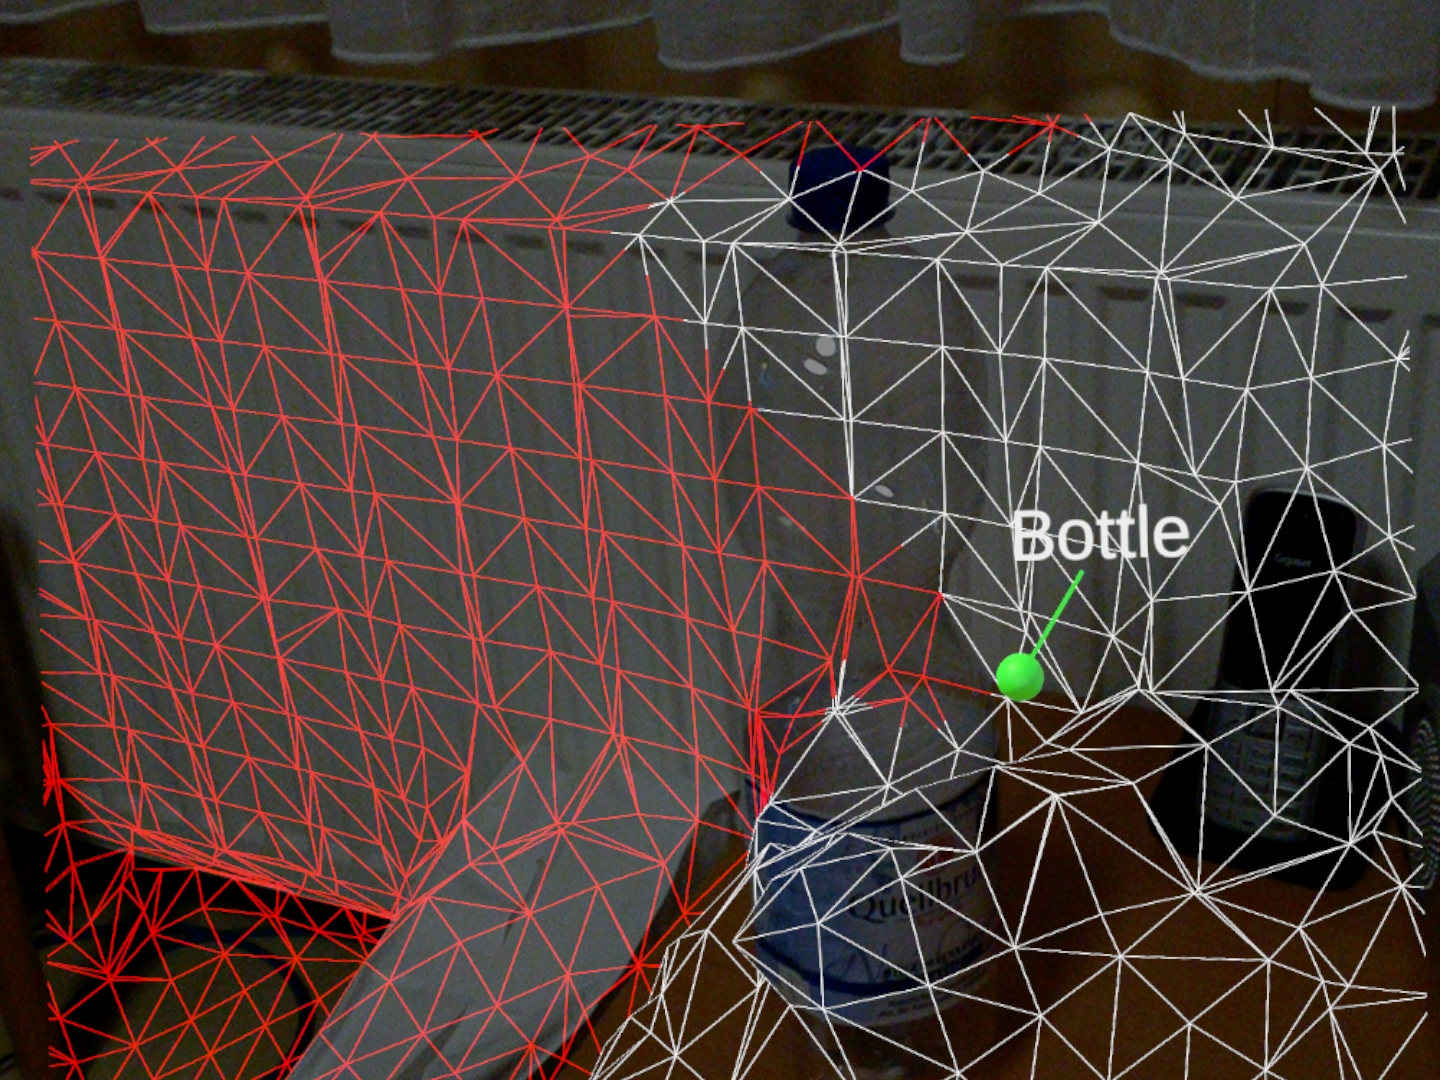
\includegraphics[width=0.8\textwidth]{images/ML_20201004_19.12.13.jpg}
	\caption[]{Label für Bottle liegt hinter dem Tatsächlichen Objekt. Die Flasse wurde nicht korrekt gemapped.}
	\label{img:flasche}
\end{figure}
